\documentclass[specialreport]{subfiles}
\begin{document}


%Qn : Hyper Cube
%Sn : Star Graph
%Pn : Pancake Graph
%BPn : Burnt Pancake Graph
%HPn : Half Pancake Graph
%Rn : Rotator Graph
%BRn : Bi Rotator Graph
%Tn : Transposition Graph
%SRn : Sustring Reversal Graph
%Bn : Bubble Sort Graph

\section{様々なケイリーグラフ}
\label{sec:variousgraphs}
本章では本レポートで取り扱う様々なケイリーグラフに関して述べる.

%hyper cube
\subsection{ハイパーキューブ (hypercube)$Q_n$}
{\vu} $=(u_1, u_2, \dots, u_n)$を$0$と$1$からなる作られるビット列とする.
整数$i (1\leq i  \leq n)$に対して記号反転操作$Q_{i}(\vu)$を次のように定義する.
\begin{equation*}
Q_{i}(\vu) = (u_1,u_2,\dots , (u_{i} + 1) ~mod~ 2,  \dots, u_n)
\end{equation*}

無向グラフ$G(V,E)$に対して$n$-hypercube $Q_n=(V, E)$の$V, E$を以下に示す.
\begin{equation*}
\begin{split}
V = ~& \{u_1u_2\dots u_n ~| 0と1からなる作られる長さnの全てのビット列\}\\
E = ~& \{(\vu,Q_i(\vu))|\vu \in V,  1 \leq i \leq n\}
\end{split}
\end{equation*}

以後$n$-ハイパーキューブ を$Q_n$とする。
図\ref{fig:4hypercube}に$n$が4の場合のハイパーキューブ を示す。
表\ref{tab:qn_prop}に$Q_n$の性質を示す。

\begin{figure}[b]
\centering
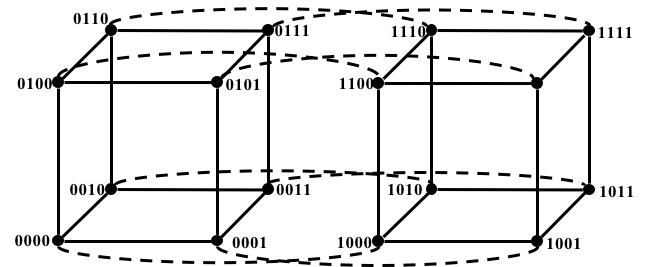
\includegraphics[width=12cm]{hypercube.png}
\caption{$4$ -ハイパーキューブ }
\label{fig:4hypercube}
\end{figure}

\begin{table}[htb]
  \begin{center}
    \caption{$n$-ハイパーキューブ の性質}
    \begin{tabular}{|c|c|c|c|c|c|c|} \hline
      単純グラフ&再帰性&対称性&頂点数&次数&連結度&直径 \\ \hline 
      yes&yes&yes&$2^n$ & $n$&$n$& $n $ \\ \hline
    \end{tabular}
    \label{tab:qn_prop}
  \end{center}
\end{table}

%star graph
\newpage
\subsection{スターグラフ(star graph)$S_n$}
{\vu} $=(u_1, u_2, \dots, u_n)$を$1$から$n$までの$n$種類の記号で作られる順列とする.
$S_j(u_1u_2\dots u_n)=u_j,u_2\dots u_{j-1}u_1u_{j+1}\dots u_n$と定義する.
無向グラフ$G(V,E)$に対して$n$-star graph $S_n=(V, E)$の$V, E$を以下に示す.
\begin{equation*}
\begin{split}
V = ~& \{u_1u_2\dots u_n ~|1,2,\dots ,n からなる全ての順列\}\\
E = ~& \{(\vu, S_i(\vu)) | u \in V, 2 \leq i \leq n )\}
\end{split}
\end{equation*}
以後$n$-スターグラフを$S_n$とする。
図\ref{fig:4stargraph}に$n$が4の場合のスターグラフを示す。表\ref{tab:sn_prop}にスターグラフの性質を示す。

\begin{figure}[b]
\centering
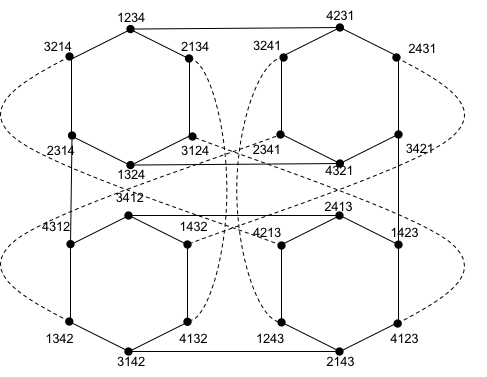
\includegraphics[width=8cm]{stargraph.png}
\caption{$4$ -スターグラフ}
\label{fig:4stargraph}
\end{figure}


\begin{table}[htb]
  \begin{center}
    \caption{$n$-スターグラフの性質}
    \begin{tabular}{|c|c|c|c|c|c|c|} \hline
      単純グラフ&再帰性&対称性&頂点数&次数&連結度&直径 \\ \hline 
      yes&yes&yes&$n!$ & $n-1$&$n-1$& $\lfloor3(n - 1) /2 \rfloor$ \\ \hline
    \end{tabular}
        \label{tab:sn_prop}
  \end{center}
\end{table}


%pancake graph
\newpage
\subsection{パンケーキグラフ(pancake graph) $P_n$}
{\vu} $=(u_1, u_2, \dots, u_n)$を$1$から$n$までの$n$種類の記号で作られる順列とする.
$PR_{i}(u_1u_2\dots u_n)=u_iu_{i-1}\dots u_1u_{i+1}u_{i+2}\dots u_n$と定義する。
無向グラフ$G(V,E)$に対して$n$-パンケーキグラフ $P_n=(V,E)$の$V, E$を以下に示す。
\begin{equation*}
\begin{split}
V = ~&\{u_1u_2\dots u_n ~|1,2,\dots ,n からなる全ての順列\}\\
E = ~&\{(\vu,PR_i(\vu)) | u \in V, 2 \leq u \leq n)\}
\end{split}
\end{equation*}
以後$n$-パンケーキグラフグラフを$P_n$とする。
図\ref{fig:4pancake}に$n$が4の場合のパンケーキグラフを示す。表\ref{tab:pn_prop}に$P_n$の性質を示す。

\begin{figure}[b]
\centering
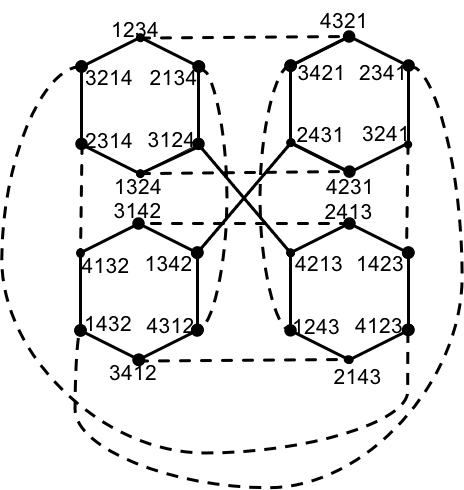
\includegraphics[width=8cm]{pancake.png}
\caption{$4$ - パンケーキグラフ}
\label{fig:4pancake}
\end{figure}


\begin{table}[htb]
  \begin{center}
    \caption{$n$-パンケーキグラフグラフの性質}
    \begin{tabular}{|c|c|c|c|c|c|c|} \hline
      単純グラフ&再帰性&対称性&頂点数&次数&連結度&直径 \\ \hline 
      yes&yes&yes&$n!$ & $n-1$&$n-1$& $ \leq \lceil 5(n + 1) /3 \rceil$ \\ \hline
    \end{tabular}
    \label{tab:pn_prop}
  \end{center}
\end{table}

%BPn : Burnt Pancake Graph
\newpage
\subsection{焦げたパンケーキグラフ(burnt pancake graph)$BP_n$}
{\vu} $=(u_1, u_2, \dots, u_n)$を$1$から$n$までの$n$種類の符号付き記号で作られる順列とする.
次に符号付き前置反転操作$SR_i(u_1u_2\dots u_n)=\overline{u_iu_{i-1}}\dots \overline{u_1}u_{i+1}u_{i+2}\dots u_n$と定義する。
無向グラフ$G(V,E)$に対して$n$-焦げたパンケーキグラフ $BP_n=(V,E)$の$V, E$を以下に示す。
\begin{equation*}
\begin{split}
V = ~& \{u_1u_2\dots u_n ~|1,2,\dots ,n からなる全ての順列\}\\
E = ~&\{(u,PR_i(u) | u \in V, 1 \leq u \leq n)\}
\end{split}
\end{equation*}

以後$n$-焦げたパンケーキグラフを$BP_n$とする。
図\ref{fig:3burntpancake}に$n$が3の場合の焦げたパンケーキグラフを示す。表\ref{tab:bpn_prop}に$BP_n$の性質を示す。
\begin{figure}[b]
\centering
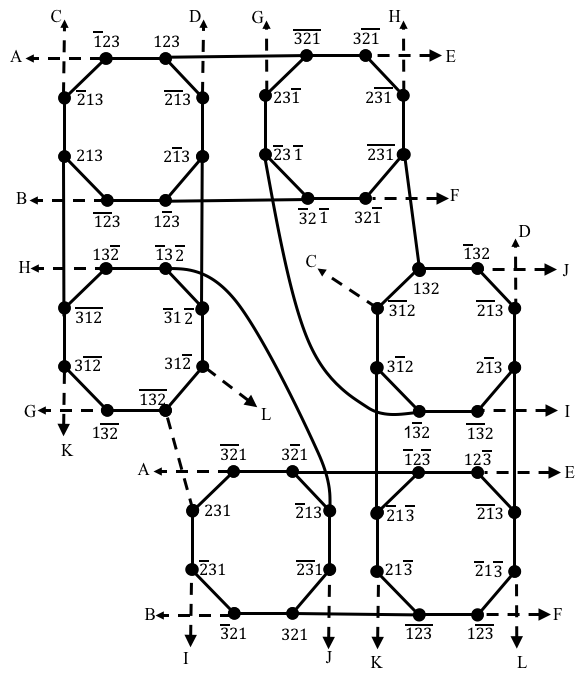
\includegraphics[width=8cm]{burntpancake.png}
\caption{$3$ - 焦げたパンケーキグラフ}
\label{fig:3burntpancake}
\end{figure}


\begin{table}[httpb]
  \begin{center}
    \caption{$n$-焦げたパンケーキグラフの性質}
    \begin{tabular}{|c|c|c|c|c|c|c|} \hline
      単純グラフ&再帰性&対称性&頂点数&次数&連結度&直径 \\ \hline 
      yes&yes&yes&$n!\times 2^{n}$ & $n$&$n$& $ \leq 2n + 3$ \\ \hline
    \end{tabular}
        \label{tab:bpn_prop}
  \end{center}
\end{table}


%Rn : Rotator Graph
\newpage
\subsection{ローテータグラフ(rotator graph)$R_n$}
{\vu} $=(u_1, u_2, \dots, u_n)$を$1$から$n$までの$n$種類の記号で作られる順列とする.
有向グラフ$G(V,E)$に対して$n$-ローテータグラフ $R_n=(V,E)$の$V, E$を以下に示す。
\begin{equation*}
\begin{split}
V = ~& \{u_1u_2\dots u_n ~|1,2,\dots ,n からなる全ての順列\}\\
E = ~& \{(\vu,\vv)|\vu \in V, \vv \in V, \vu=(u_1, u_2, \dots u_n), \vv=(v_1, v_2, \dots v_n) の場合\\
&\vu に対して\vu から\vv への有向辺が\\
&v_1 = u_2, v_2 = u_3, \dots , v_{i-1} = u_i , v_i = u_1 , v_{i+1} = u_{i+1} , \\
&\dots , v_n = u_n \ を満たす i (2 \leq i \leq n) があれば存在\}
\end{split}
\end{equation*}
以後$n$-ローテータグラフを$R_n$とする。
図\ref{fig:3rotator}に$n$が3の場合のローテータグラフを示す。表\ref{tab:rn_prop}に$R_n$の性質を示す。

\begin{figure}[b]
\centering
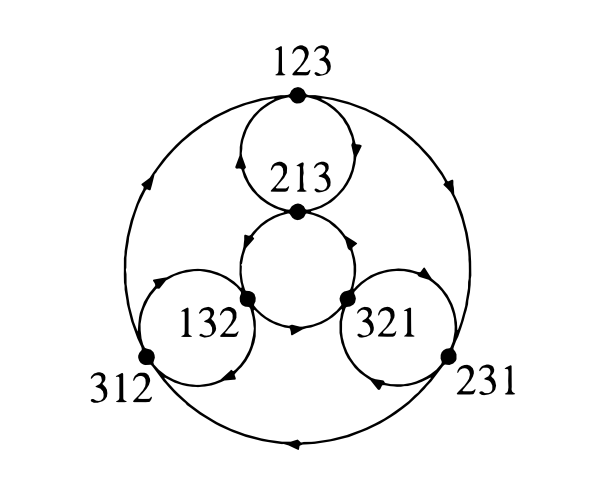
\includegraphics[width=8cm]{rotatorgraph.png}
\caption{$3$ - ローテータグラフ}
\label{fig:3rotator}
\end{figure}


\begin{table}[htb]
  \begin{center}
    \caption{$n$-ローテータグラフの性質}
    \begin{tabular}{|c|c|c|c|c|c|c|} \hline
      単純グラフ&再帰性&対称性&頂点数&次数&連結度&直径 \\ \hline 
      yes&yes&yes&$n!$ & $n-1$&$n-1$& $ n-1 $ \\ \hline
    \end{tabular}
    \label{tab:rn_prop}
  \end{center}
\end{table}



%BRn : Bi Rotator Graph
\newpage
\subsection{バイローテータグラフ(rotator graph)$BR_n$}
{\vu} $=(u_1u_2 \dots u_n)$を$1$から$n$までの$n$種類の記号で作られる順列とする.
整数$i (2\leq i \leq n)$に対して正のローテーション操作$R^{+}_{i}(\vu)$と負のローテーション操作$R^{-}_{i}(\vu)$を
次のように定義する.
\begin{equation*}
\begin{split}
R^{+}_{i}(\vu) = & (u_2, u_3, \dots, u_i, u_1, u_{i+1}, u_{i+2}, \dots, u_n)\\
R^{-}_{i}(\vu) = &(u_i, u_1, u_2, \dots, u_{i-1}, u_{i+1}, u_{i+2}, \dots, u_n)
\end{split}
\end{equation*}
有向グラフ$G(V,E)$に対して$n$-バイローテータグラフ $BR_n=(V,E)$の$V, E$を以下に示す。
\begin{equation*}
\begin{split}
V = ~& \{u_1u_2\dots u_n ~|1,2,\dots ,n からなる全ての順列\}\\
E = ~& \{(\vu,\vv)|\vu \in V,\vv \in V, \vv=R^{+}_{i}(\vu) ~or~ \vv = R^{-}_{i}(\vu) , 2 \leq i \leq n\}
\end{split}
\end{equation*}
以後$n$-バイローテータグラフを$BR_n$とする。
図\ref{fig:3birotator}に$n$が3の場合のローテータグラフを示す。表\ref{tab:brn_prop}に$BR_n$の性質を示す。

\begin{figure}[b]
\centering
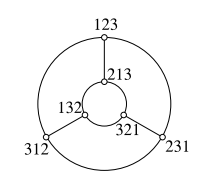
\includegraphics[width=8cm]{birotatorgraph.png}
\caption{$3$ - バイローテータグラフ}
\label{fig:3birotator}
\end{figure}


\begin{table}[htb]
  \begin{center}
    \caption{$n$-バイローテータグラフの性質}
    \begin{tabular}{|c|c|c|c|c|c|c|} \hline
      単純グラフ&再帰性&対称性&頂点数&次数&連結度&直径 \\ \hline 
      yes&yes&yes&$n!$ & $2n-3$&$2n-3$& $ n-1 $ \\ \hline
    \end{tabular}
    \label{tab:brn_prop}
  \end{center}
\end{table}



%Tn : Transposition Graph
\newpage
\subsection{トランスポジショングラフ(transpostion graph)$T_n$}
{\vu} $=(u_1, u_2, \dots, u_n)$を$1$から$n$までの$n$種類の記号で作られる順列とする.
整数$i, j  (1\leq i < j  \leq n)$に対してトランスポジション操作$T{i,j}(\vu)$を次のように定義する.
\begin{equation*}
T_{i,j}(\vu) = (u_1,u_2,\dots ,u_{i-1}, u_{j}, u_{i+1}, \dots, u_{j-1}, u_i,  u_{j+1}, \dots, u_n)
\end{equation*}
無向グラフ$G(V,E)$に対して$n$-トランスポジショングラフ $T_n=(V,E)$の$V, E$を以下に示す。
\begin{equation*}
\begin{split}
V = ~& \{u_1u_2\dots u_n ~|1,2,\dots ,n からなる全ての順列\}\\
E = ~& \{(\vu, T_{i,j}(\vu))|\vu \in V,  1 \leq i < j \leq n\}
\end{split}
\end{equation*}
以後$n$-トランスポジショングラフを$T_n$とする。
図\ref{fig:4transposition}に$n$が4の場合のトランスポジショングラフを示す。
表\ref{tab:tn_prop}に$T_n$の性質を示す。

\begin{figure}[b]
\centering
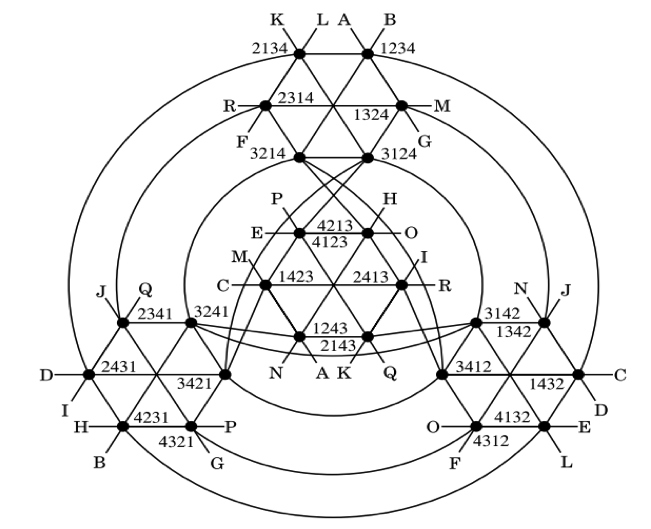
\includegraphics[width=8cm]{transpostiongraph.png}
\caption{$4$ - トランスポジショングラフ}
\label{fig:4transposition}
\end{figure}


\begin{table}[htb]
  \begin{center}
    \caption{$n$-トランスポジショングラフの性質}
    \begin{tabular}{|c|c|c|c|c|c|c|} \hline
      単純グラフ&再帰性&対称性&頂点数&次数&連結度&直径 \\ \hline 
      yes&yes&yes&$n!$ & $n(n-1)/2$&$n(n-1)/2$& $ n-1 $ \\ \hline
    \end{tabular}
    \label{tab:tn_prop}
  \end{center}
\end{table}

%SRn : Sustring Reversal Graph
\newpage
\subsection{部分文字列反転グラフ(substring reversal graph) $SR_n$}
{\vu} $=(u_1u_2 \dots u_n)$を$1$から$n$までの$n$種類の記号で作られる順列とする.
整数$i, j  (1\leq i < j  \leq n)$に対して部分文字列反転操作$SR_{i,j}(\vu)$を次のように定義する.
\begin{equation*}
SR_{i,j}(\vu) = (u_1,u_2,\dots ,u_{i-1}, u_{j}, u_{j-1}, \dots, u_{i+1}, u_i,  u_{j+1}, \dots, u_n)
\end{equation*}
無向グラフ$G(V,E)$に対して$n$-部分文字列反転グラフ $SR_n=(V,E)$の$V, E$を以下に示す。
\begin{equation*}
\begin{split}
V = ~& \{u_1u_2\dots u_n ~|1,2,\dots ,n からなる全ての順列\}\\
E = ~& \{(\vu , SR_{i,j}(\vu))|\vu \in V, 1 \leq i < j \leq n\}
\end{split}
\end{equation*}
以後$n$-部分文字列反転グラフを$SR_n$とする。
図\ref{fig:4substringreversalgraph}に$n$が4の場合の部分文字列反転グラフを示す。
表\ref{tab:srn_prop}に$SR_n$の性質を示す。

\begin{figure}[b]
\centering
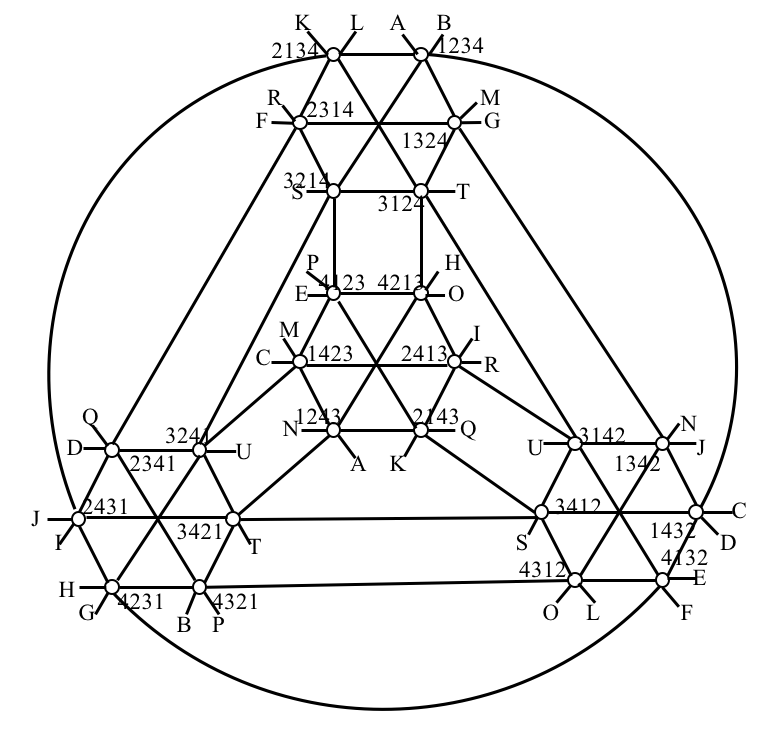
\includegraphics[width=8cm]{substringreversalgraph.png}
\caption{$4$ - 部分文字列反転グラフ}
\label{fig:4substringreversalgraph}
\end{figure}


\begin{table}[htb]
  \begin{center}
    \caption{$n$-部分文字列反転グラフの性質}
    \begin{tabular}{|c|c|c|c|c|c|c|} \hline
      単純グラフ&再帰性&対称性&頂点数&次数&連結度&直径 \\ \hline 
      yes&yes&yes&$n!$ & $(n-1)(n-2)/2$&$(n-1)(n-2)/2$& $\leq n-1 $ \\ \hline
    \end{tabular}
    \label{tab:srn_prop}
  \end{center}
\end{table}

%Bn : Bubble Sort Graph
\newpage
\subsection{バーブルソートグラフ(bubble sort graph) $B_n$}
{\vu} $=(u_1, u_2, \dots, u_n)$を$1$から$n$までの$n$種類の記号で作られる順列とする.
整数$i (1\leq i  \leq n - 1)$に対して隣接交換操作$B_{i}(\vu)$を次のように定義する.
\begin{equation*}
B_{i}(\vu) = (u_1,u_2,\dots ,u_{i-1}, u_{i+1}, u_{i},  u_{i+1}, \dots, u_n)
\end{equation*}
無向グラフ$G(V,E)$に対して$n$-バーブルソートグラフ $B_n=(V,E)$の$V, E$を以下に示す。
\begin{equation*}
\begin{split}
V = ~& \{u_1u_2\dots u_n ~|1,2,\dots ,n からなる全ての順列\}\\
E = ~& \{(\vu,B_i(\vu))|\vu \in V,  1 \leq i \leq n-1\}
\end{split}
\end{equation*}


以後$n$-バーブルソートグラフを$B_n$とする。
図\ref{fig:4bubblesortgraph}に$n$が4の場合のバーブルソートグラフを示す。
表\ref{tab:bn_prop}に$B_n$の性質を示す。

\begin{figure}[b]
\centering
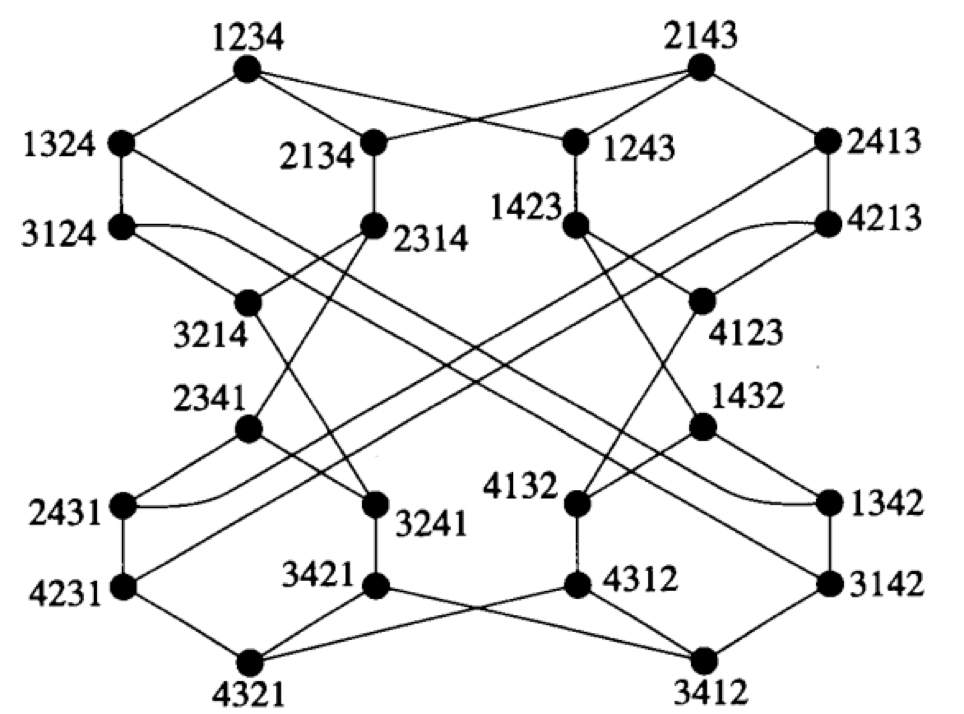
\includegraphics[width=8cm]{bubblesortgraph.png}
\caption{$4$ -バーブルソートグラフ }
\label{fig:4bubblesortgraph}
\end{figure}


\begin{table}[htb]
  \begin{center}
    \caption{$n$-バーブルソートグラフの性質}
    \begin{tabular}{|c|c|c|c|c|c|c|} \hline
      単純グラフ&再帰性&対称性&頂点数&次数&連結度&直径 \\ \hline 
      yes&yes&yes&$n!$ & $n-1$&$n-1$& $(n-1)n/2 $ \\ \hline
    \end{tabular}
    \label{tab:bn_prop}
  \end{center}
\end{table}










\end{document}